\section{Spoken Language Understanding (SLU)}
\begin{frame}{}
    \LARGE \textbf{Spoken Language Understanding (SLU)}
\end{frame}


\begin{frame}[allowframebreaks]{Spoken Language Understanding (SLU)}

\begin{itemize}
    \item SLU focuses on understanding the meaning of spoken utterances, going beyond mere transcription.  
    \item Goal: transform ``what was said'' → ``what was meant.''

    \item Input and output:
    \begin{itemize}
        \item Input: audio signal.
        \item Output: structured meaning, typically \textbf{intent + slots}.
    \end{itemize}

    \item Definitions:
    \begin{itemize}
        \item \textbf{Intent:} the action the user wants to perform (e.g., play music, set an alarm).
        \item \textbf{Slots:} arguments of the intent (e.g., \{song: ``Yesterday'', artist: ``Beatles''\}).
    \end{itemize}
\framebreak
    \item Example:
    \begin{itemize}
        \item Audio: ``Set an alarm for 7 a.m.''  
        \item Output: \{intent: set\_alarm, time: 7:00\}
    \end{itemize}

    \item Why SLU is important:
    \begin{itemize}
        \item Enables interaction with smart assistants and dialogue systems.
        \item Bridges the gap between raw speech signals and actionable NLP tasks.
    \end{itemize}
\end{itemize}

    \begin{figure}
        \centering
        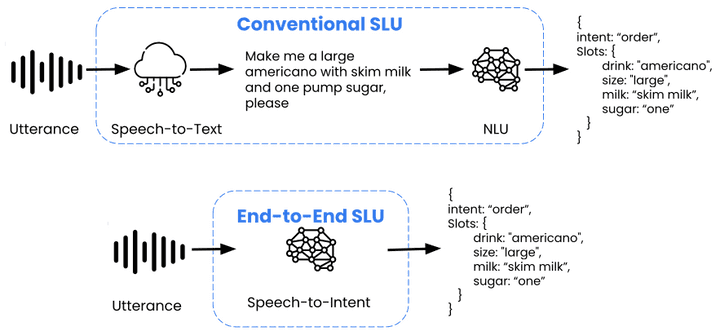
\includegraphics[width=\textwidth,height=0.8\textheight,keepaspectratio]{images/audio-nlp-eval/slu-diagram.png}
        \caption*{Spoken Language Understanding. Source: \href{https://picovoice.ai/blog/spoken-language-understanding-slu/}{PICOVOICE.AI}}
    \end{figure}

\end{frame}


\begin{frame}[allowframebreaks]{SLU Pipeline (ASR → NLU)}

\begin{itemize}
    \item Many commercial SLU systems follow a two-step pipeline, separating speech recognition from understanding.

    \item Pipeline steps:
    \begin{enumerate}
        \item \textbf{Audio → ASR → Text Transcript}  
        Converts raw audio into written words.
        
        \item \textbf{Text → NLU Model}  
        \begin{itemize}
            \item \textbf{Intent classification:} identifies user’s action (e.g., \texttt{request\_weather}).  
            \item \textbf{Slot filling:} extracts entities or arguments (e.g., \{location: ``London''\}).
        \end{itemize}
        
        \item \textbf{Dialogue manager:} decides system response or action based on intent and slots.
    \end{enumerate}
\framebreak
    \item Advantages of this approach:
    \begin{itemize}
        \item Leverages existing NLP models trained on text.
        \item Easier to build and maintain using large text corpora.
    \end{itemize}

    \item Example:
    \begin{itemize}
        \item User says: ``What’s the weather like in Paris?''  
        \item ASR output: ``what’s the weather like in paris''  
        \item NLU output: \{intent: get\_weather, location: ``Paris''\}
    \end{itemize}
\end{itemize}

\end{frame}


\begin{frame}[allowframebreaks]{Direct SLU (End-to-End)}

\begin{itemize}
    \item Direct SLU models bypass transcription and predict meaning directly from audio signals.

    \item How it works:
    \begin{itemize}
        \item Input features: log-Mel spectrograms or wav2vec embeddings.
        \item Model architecture: typically CNNs or Transformers for classification or sequence labeling.
        \item Output: intent + slots, directly mapped from audio.
    \end{itemize}
\framebreak
    \item Advantages:
    \begin{itemize}
        \item Avoids error propagation from ASR mistakes.
        \item Ideal for domain-specific commands where transcription is unnecessary.
        \item Faster and more efficient than pipeline approaches.
    \end{itemize}

    \item Example:
    \begin{itemize}
        \item Audio: ``Play jazz''  
        \item Direct SLU output: \{intent: play\_music, genre: ``jazz''\}  
        \item No intermediate transcript is generated.
    \end{itemize}
\end{itemize}

\end{frame}


\begin{frame}[allowframebreaks]{Challenges in SLU}

\begin{itemize}
    \item Spoken Language Understanding faces several real-world challenges:

    \item \textbf{Error Propagation:}  
    In pipeline systems, ASR mistakes can cause NLU errors.  
    \textit{Example:} ``Play rock'' misheard as ``Play doc'' → system fails.

    \item \textbf{Data Scarcity:}  
    Annotated SLU datasets are often small. Collecting paired (speech, intent, slots) data is expensive.

    \item \textbf{Multilinguality & Code-Switching:}  
    Users often mix languages in the same utterance.  
    \textit{Example:} ``Ponme una canción by Shakira.''  
    Systems must handle hybrid language input robustly.

    \item \textbf{Context & Dialogue:}  
    Understanding multi-turn conversations requires memory of previous interactions.  
    \textit{Example:} ``Play jazz.'' → ``Now make it louder.''
\end{itemize}

\end{frame}


\begin{frame}[allowframebreaks]{Applications of SLU}

\begin{itemize}
    \item Spoken Language Understanding powers many real-world applications by extracting meaning from speech, not just transcribing it.

    \item Common use cases:
    \begin{itemize}
        \item \textbf{Virtual assistants:} Siri, Alexa, Google Assistant.
        \item \textbf{Smart homes:} voice-controlled lights, appliances.
        \item \textbf{Customer service:} routing calls based on intent.
        \item \textbf{Automotive:} navigation, calls, climate control.
        \item \textbf{Healthcare:} converting doctors’ spoken notes into structured forms.
    \end{itemize}
\framebreak
    \item Example (Alexa):
    \begin{itemize}
        \item User says: ``Turn off the bedroom lights.''  
        \item SLU output: \{intent: control\_device, device: lights, location: bedroom\}
    \end{itemize}

    \item Why SLU is critical:
    \begin{itemize}
        \item Transcription alone isn’t sufficient; systems must act on the meaning of what was said.
    \end{itemize}
\end{itemize}

\end{frame}
